
%\begin{figure}[t]
%	\centering
%	\begin{minipage}{0.28\textwidth}
%		\centering
%		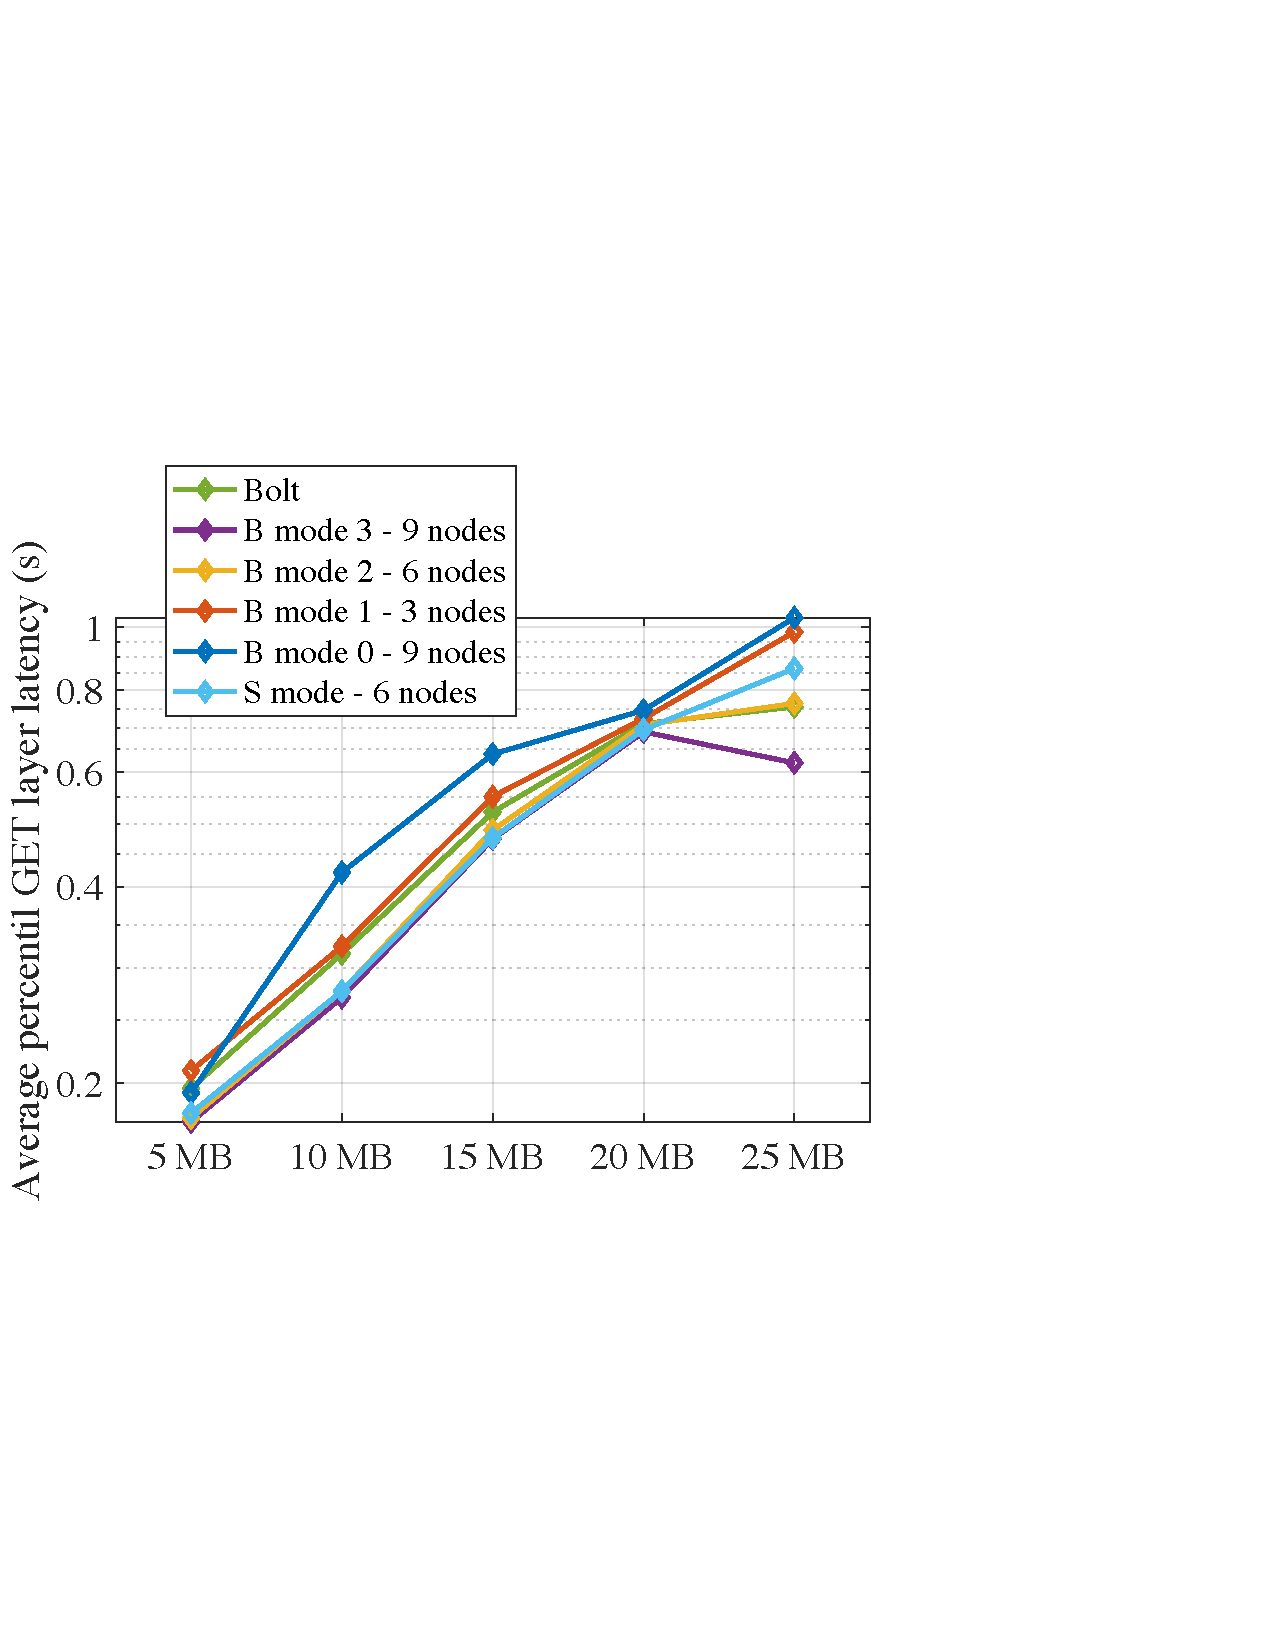
\includegraphics[width=0.9\textwidth]{graphs/dalprimaryperformance.pdf}
%		\caption{GET layer latency.\todo{add grid in background to match the other figures}}% across different schemes.}
%		\label{fig:eval-1nodegetlayerlatency}
%	\end{minipage}%
%	\begin{minipage}{0.28\textwidth}
%		\centering
%		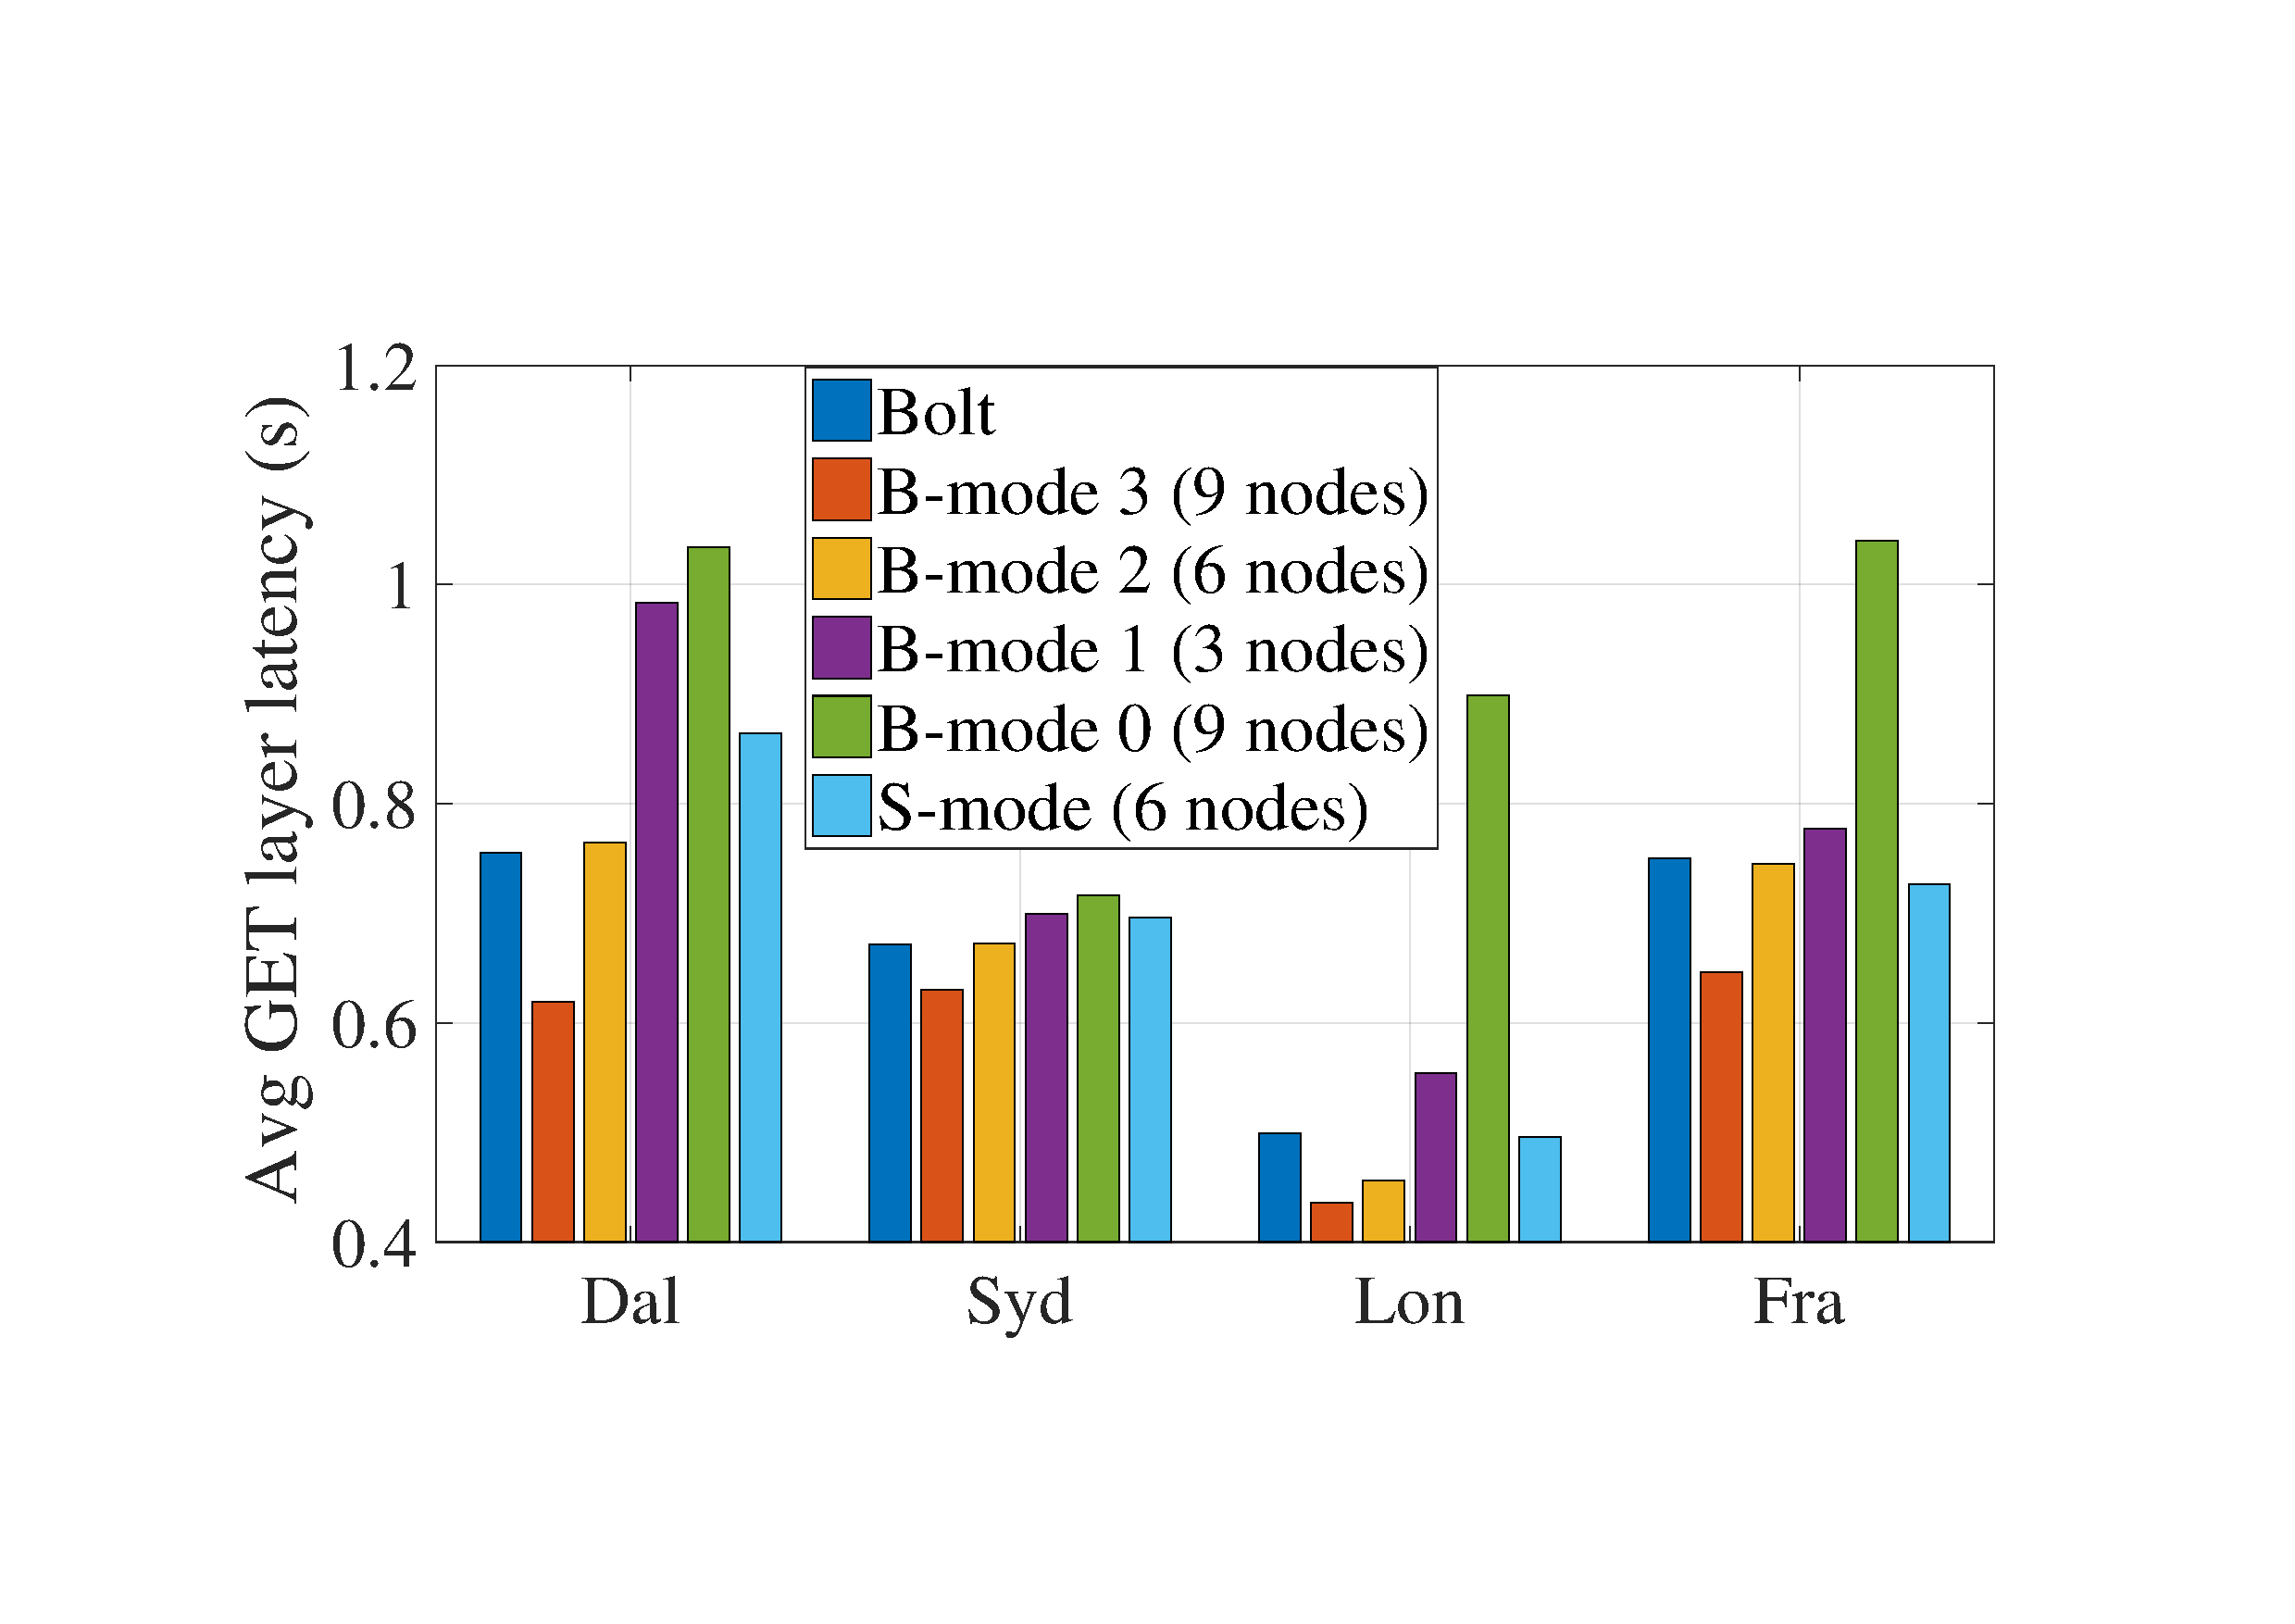
\includegraphics[width=0.9\textwidth]{graphs/total-traces.pdf}
%		\caption{Cache hit ratio.}% of LRU cache and preconstruct cache.}
%		\label{fig:eval-cachehitratios}
%	\end{minipage}%
%%	\begin{minipage}{0.3\textwidth}
%%	\centering
%%	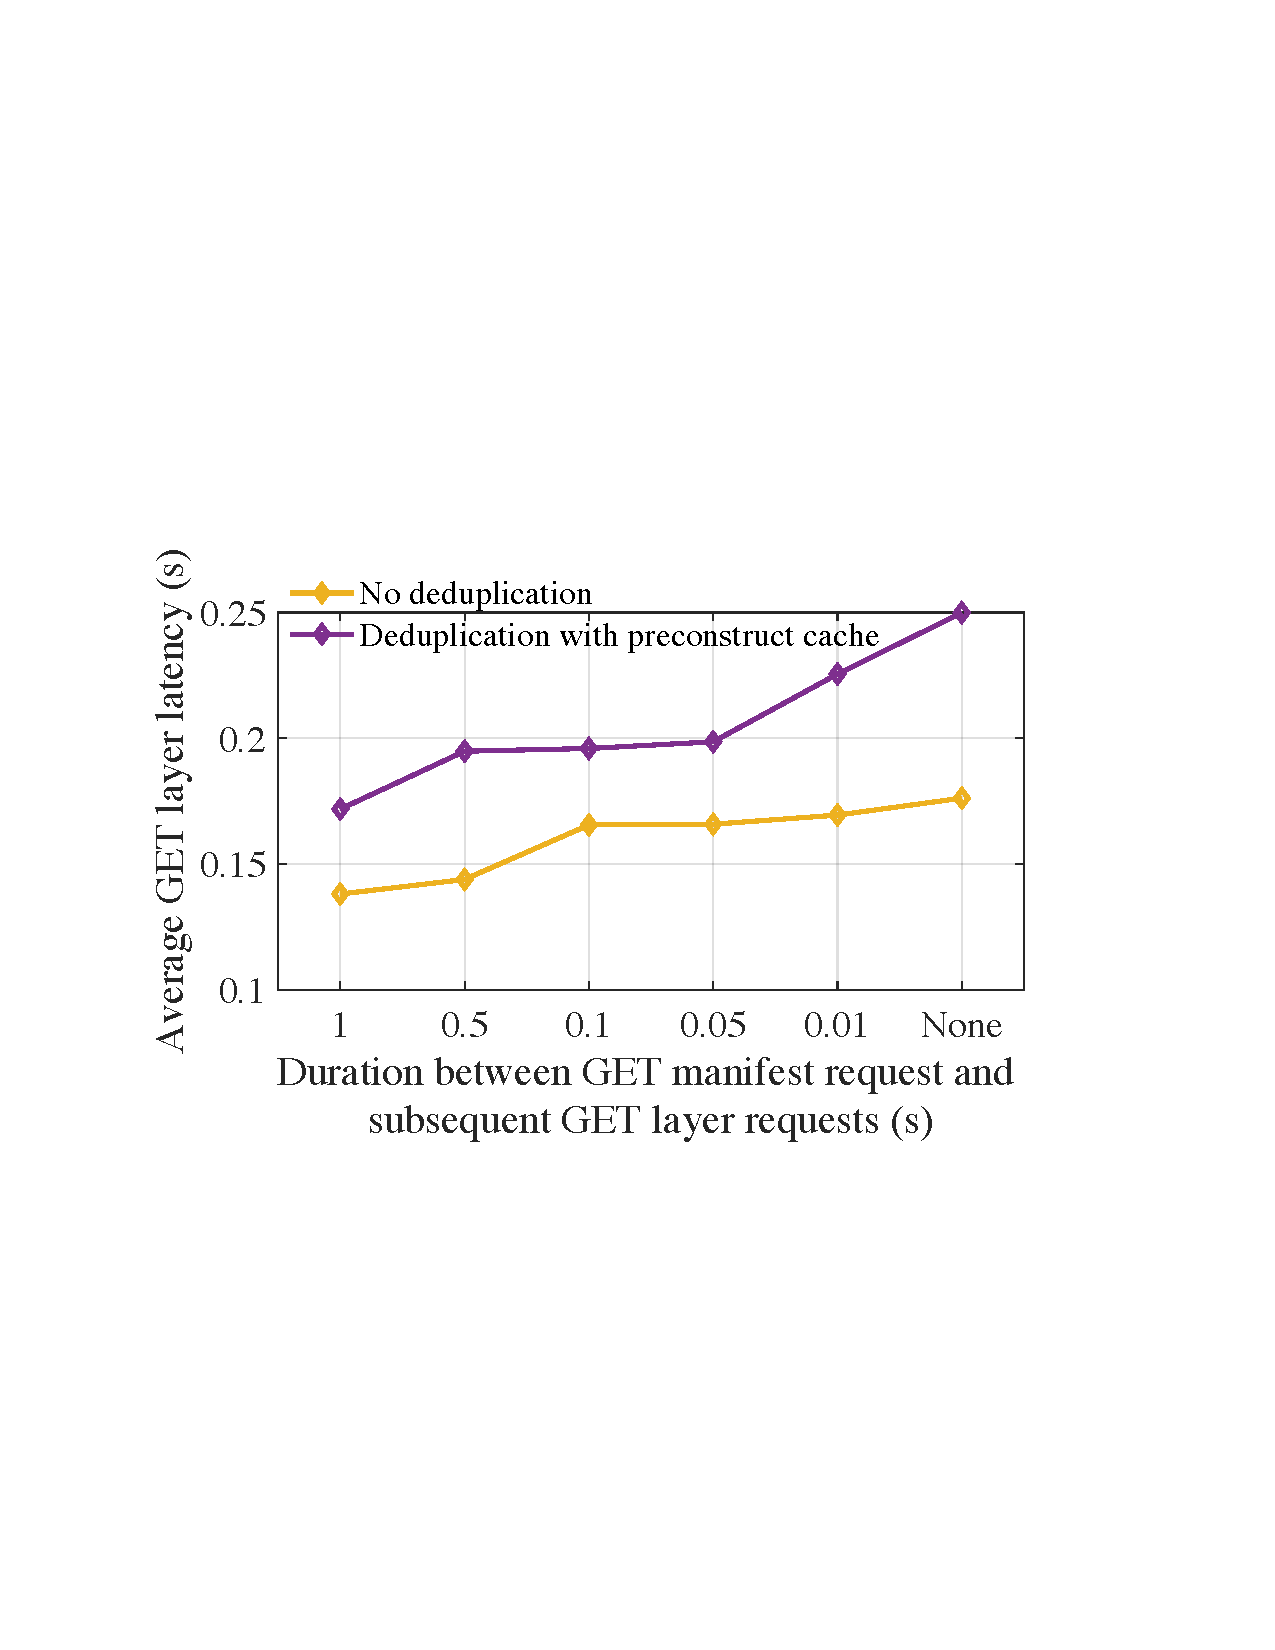
\includegraphics[width=0.9\textwidth]{graphs/durationML.pdf}
%%	\caption{The impact of durationML.}
%%	\label{fig:eval-durationML}
%%   \end{minipage}
%
%\end{figure}


\begin{figure}[t]
	\centering
	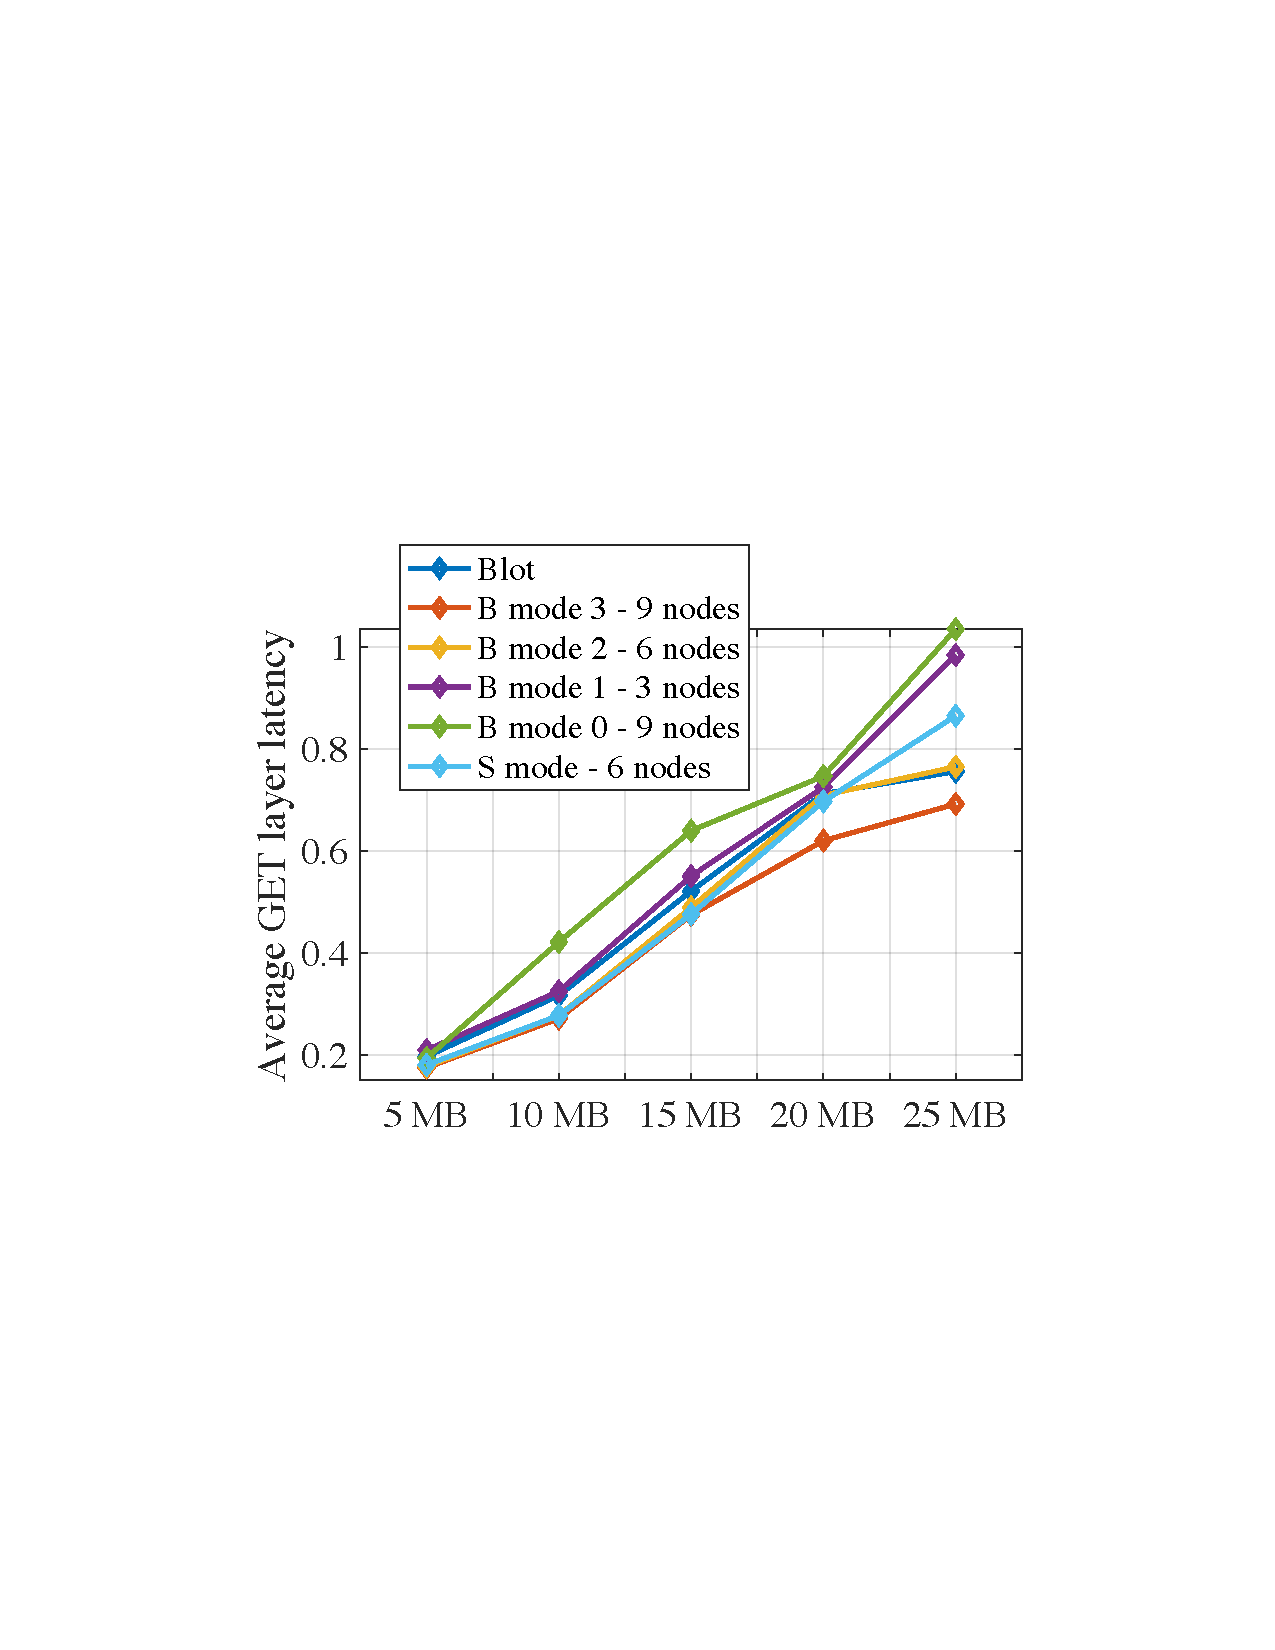
\includegraphics[width=0.4\textwidth]{graphs/dalprimary.pdf}
	\caption{Average \texttt{GET} layer latency.}
	%	\vspace{-3pt}
	\label{fig:eval-dalprimary}
	
\end{figure}

\begin{figure}[t]
	\centering
	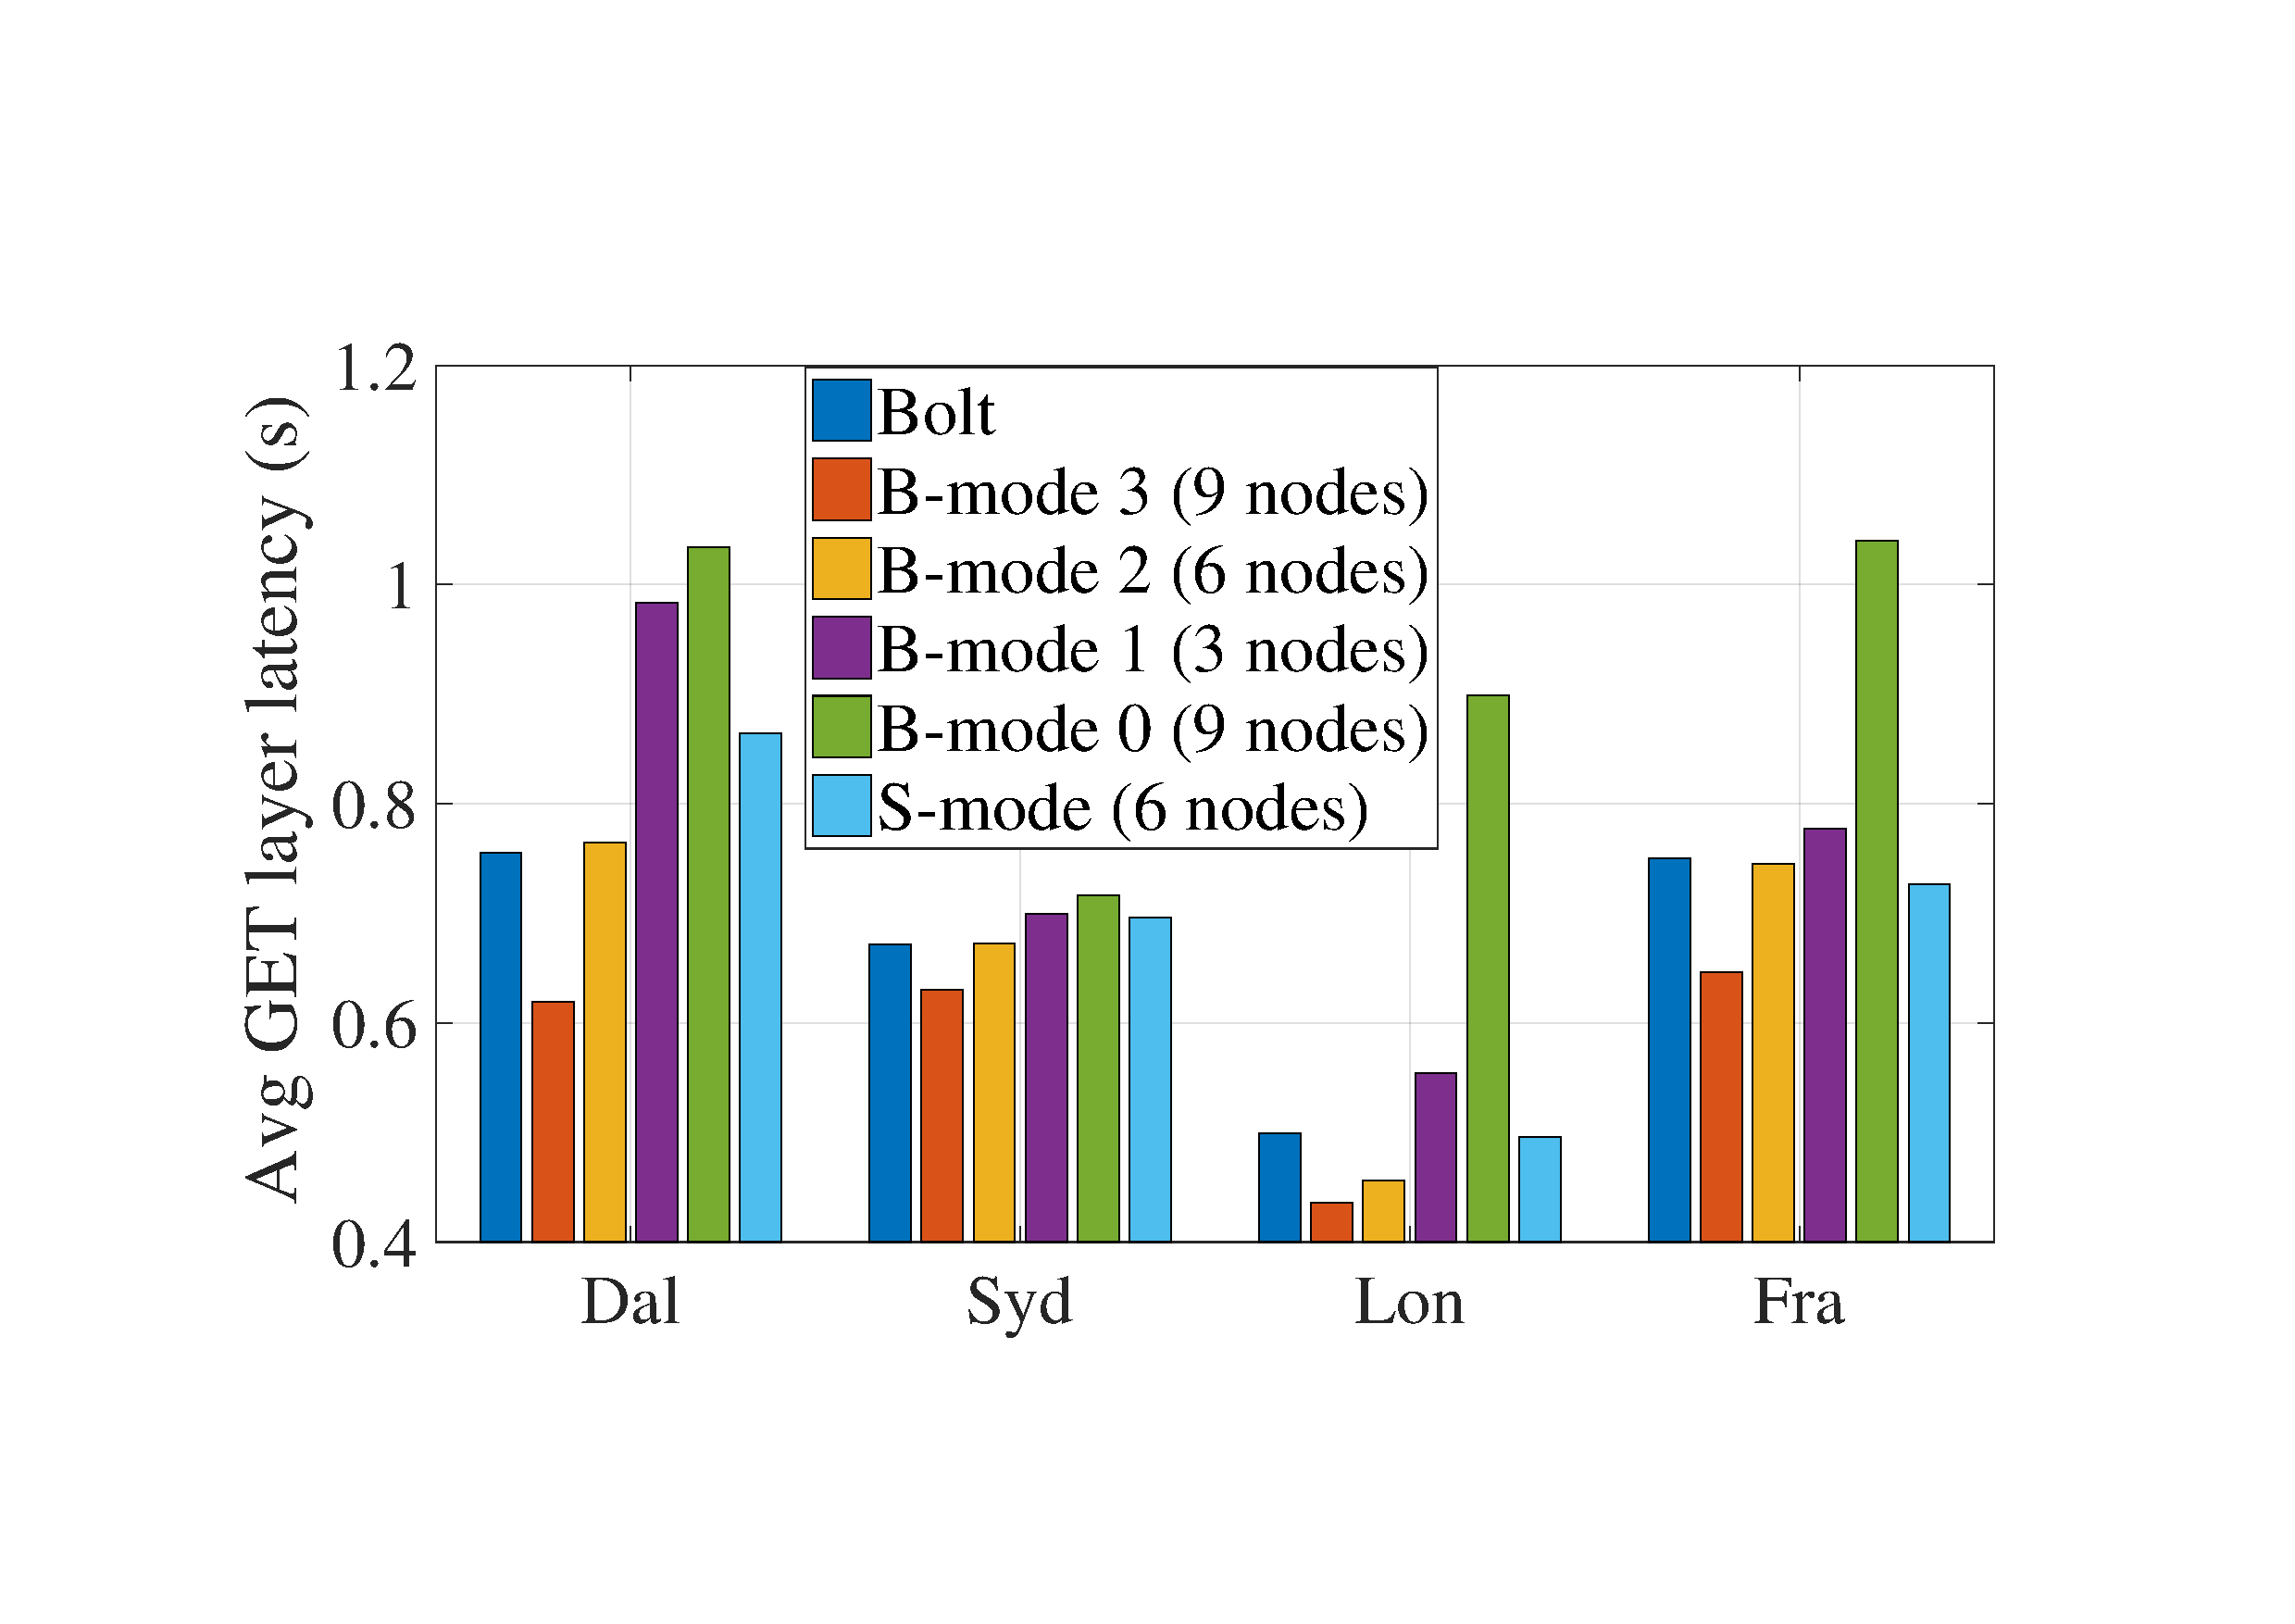
\includegraphics[width=0.4\textwidth]{graphs/total-traces.pdf}
	\caption{Average \texttt{GET} layer latency.} %\Subil{"Blot" in figure should be "BOLT".}}
	%	\vspace{-3pt}
	\label{fig:eval-total-traces}
	
\end{figure}


\begin{table}[]
		\scriptsize
	\begin{tabular}{ | l | l | l | }
		\hline
	                	     & Dedup ratio & layer restoring latency increases \\ \hline
	 \multicolumn{3}{|c|}{********* File level [3-way replication] *********} \\ \hline
	B-mode 0	       &          2 x           &  \\ \hline
	B-mode 1            &          1.5 x           &  \\ \hline
	B-mode 2	       &           1.2 x            &  \\ \hline
%	B-mode 3	       &                        &  \\ \hline
	S-mode  	          &           1.3 x             &  \\ \hline
	 \multicolumn{3}{|c|}{********* Block level [3-way replication] *********} \\ \hline
	B-mode 0 	       &        4 x             &  \\ \hline
	B-mode 1            &        2 x             &  \\ \hline
	B-mode 2	       &         1.3 x              &  \\ \hline
%	B-mode 3	       &                        &  \\ \hline
	S-mode  	          &          1.7 x              &  \\ \hline
	 \multicolumn{3}{|c|}{********* Block level [Erasure coding] *********} \\ \hline
	B-mode 0 	  &           6 x             &  \\ \hline
	\end{tabular}
\end{table}


\subsection{Deduplication Modes}
\label{sec:eval-primary}
%\paragraph{}
Next, we evaluate the performance of \sysname's primary cluster
and different B-mode configurations.
%
We test five modes of \sysname on a 9-node cluster: B-mode 0, 1, 2, and 3,
and S-mode.
%
B-mode 0 deduplicates \emph{all} layer replicas while B-mode 3 does not perform deduplication.
%\sysname is evaluated by configuring different deduplication modes.
%
Accordingly, B-mode 0 doesn't have P-servers while B-mode 3 doesn't have D-servers.
%
For the remaining two B-modes, B-mode 1 and B-mode 2, the number of P-servers
is set to 3 and 6, respectively. For S-mode, the number of P-servers is set to 6.
%In addition, 
%we speedup trace replaying by using different speedup factors
%so that each trace can be finished within 30 minutes.
%Before we replay each workload, 
%we first warmup P-servers and D-servers with a certain amount of layers 
%as shown in Table~\ref{tab:eval-overall}, which roughly takes 10 minutes.
%To generate workload, 
%
We use 100 clients to replay the traces and BOLT with 3-way replication on the same 9-node setup as our baseline. 

%\LR{What does it mean that we're varying the layer size?}
%
\paragraph{Different layer sizes} Figure~\ref{fig:eval-dalprimary} shows the average \texttt{GET} layer response
for the \dal workload, varying the layer size (from 5\,MB to 25\,MB).
%
Note that for B-mode 0, the \texttt{GET} layer latency refers to the
layer restoring latency as no complete layer replica is stored.

%Overall, \texttt{PUT} requests have much higher average response time than \texttt{GET} requests.
%For example, the average response time of 
%\texttt{PUT} layer requests is almost twice higher than that of \texttt{GET} layer requests.
%Note that registry servers use SSDs as secondary storage devices.
%The difference in response time for \texttt{PUT} and \texttt{GET} requests are mainly caused by the different writes and reads throughput of SSDs. 

%Our first observation is that the average \texttt{GET} layer latency increases with layer size for all the schemes.
%%
%For example, when the layer size increases from 5~MB to
%25~MB, the average \texttt{GET} layer latency for \emph{BOLT} grows from 0.19~s
%to 0.7~s, and from 0.17~s to 0.6~s for \emph{B-mode 3}.
%%
%Moreover, when the
%layer size is 5~MB, the average \texttt{GET} layer latency across the
%schemes is around 0.2~s with minimal variation.
%\DIM{Although it's true that 5MB has the smallest variation, it seems to me that only 25MB has any significant variation. Can you given any insight as to why?}
%%
%For example, the
%lowest and highest \texttt{GET} layer latency when the layer size is 5~MB are
%0.17~s and 0.21~s for \emph{B-mode 3} and \emph{B-mode 1}, respectively.

As expected, the response times increase with a larger layer size for all configurations.
%
Overall, B-mode 3 achieves the lowest latencies as it is not performing any deduplication.
%
Compared to BOLT, B-mode 3 benefits from \sysname{}'s superfetch cache, which
lowers latencies by prefetching layers into and serving them from memory.
%
B-mode 3 is able to reduce the average \texttt{GET} latencies by 13\% compared to
BOLT for a layer size of 20\,MB.
%\DIM{The 13\% is not significant by itself. Is there some other benefit of mode3 over BOLT, like space savings, that could be added here?}
%
The superfetch cache hit ratio in this case is 0.91.
%
%However, the network transfer time accounts for the largest portion of
%the \text{GET} layer latency for \emph{BOLT} and \emph{B-mode 3}.
%\DIM{how much is that portion?}

Looking at B-mode 0, we see that it adds the highest overhead, up to 37\%, to
the \texttt{GET} layer latencies as it deduplicates everything and maximizes
storage savings.
%
%Next we compare \emph{B-mode 0} with \emph{BOLT}.
%
%Although \emph{B-mode 0} saves half of the storage space by \emph{deduplicating} all layer replicas (see
%\S\ref{sec:inter-layer-deduplication}), it increases the \texttt{GET}
%layer latency by up to 37\% due to the layer restoring overhead.
%This is because of the high preconstruct cache hit ratio (detailed in
%Figure~\cite{xxx}), which reduces the layer restoring latency.
%
The remaining B-modes are in between with B-mode 1 showing slightly higher
latencies compared to B-mode 2 as B-mode 1 only keeps one complete layer
replica.
%
Additionally, B-mode 1 only has 3 P-servers, which intensifies the load on
the primary cluster.
%
%\DIM{This is just due to the setup though? Does it tell us anything fundamental about Sift?}
%
While the difference is minor for layer sizes less than or equal to 20\,MB, only
up to 18\%, it is around 30\% for 25\,MB layers.

%basic modes: \emph{B-mode 2} and \emph{B-mode 1}, we see that
%\emph{B-mode 1} has a higher \texttt{GET} layer latency than \emph{B-mode 2}.
%
%For example, the average \texttt{GET} layer latency for \emph{B-mode 1} is 30\%
%higher than that for \emph{B-mode 2}.
%although the primary cluster of \emph{B-mode 1} only has 14 nodes while 
%\emph{original} contains 21 nodes.
%This is because only a one-third of the %less data (1/3) 
%data is \texttt{pushed} onto the primary cluster in \emph{B-mode 1}.
%\texttt{Push} requests also affect the performance of \texttt{pull} requests
%in terms of more network traffic and more writes to SSDs.
%While \emph{B-mode 2} degrades \emph{GET} layer performance by 11\%.
%This is because the primary cluster for \emph{B-mode 1} is half the \emph{B-mode 2}
%cluster and this intensifies the servers load for \emph{B-mode 1}
%causing a lot of overhead.
%\Ali{Above statement is not clear.}
%\DIM{This is just due to the setup though? Does it tell us anything fundamental about Sift?}
%For \emph{B mode 1} which has a 3-node primary cluster, more \texttt{GET}
%layer requests are sent to the P-servers, which causes a lot of overhead.
%
The \texttt{GET} layer performance of S-mode is similar to that of \emph{B-mode 2}, e.g.,
the average \texttt{GET} layer latency variation between the two modes is only
3\% when the layer size is 20\,MB.
%
This is because in S-mode, the popular layers have multiple replicas
across the 6-node cluster, which improves the overall performance.
%
Additionally, S-mode can reduce storage consumption by 40\% compared to
B-mode 2 as less popular layers keep less complete replicas.
%\NZ{s-mode saves 40\% of space.
%B-mode 2 saves 33\% of space.
%B-mode 1 saves 17\% of space.
%B-mode 0 saves 50\% of space.}
%
%However, for 25\,MB layers, the gap between S-mode and B-mode 2 widens
%because \todo{fill in reason}.
%\NZ{an error, fixed in new figure. B-mode 2 and S-mode are similar.}
%while the remaining cold layers only have a single layer replica on the
%primary cluster. 

%We find that
%\emph{B-mode 1}, \emph{B-mode 2}, \emph{B-mode 0}, and \emph{S-mode}
% also improve the \texttt{PUT} layer performance by $\sim$ 30\% as \emph{B-mode 3}.
%This is because
%all 4 modes reduce the amount of \emph{pushed} layers to primary cluster results in
%less network traffic and uses in-memory superfetch cache to reduce disk I/Os.
%Similarly,
%all modes improve \texttt{GET} and \texttt{PUT} manifest performance.
%For example, \emph{B-mode 1} reduces \texttt{GET} and \texttt{PUT}
%manifest latency by 17\% and 24\% respectively.

\paragraph{Different traces} Next, we replay all four traces from the IBM registry deployments
with a layer size of $\sim$25\,MB for all the requests.
%
%\Ali{I reworded the above statement but it still needs to be fixed.}
%
Figure~\ref{fig:eval-total-traces} shows the average \texttt{GET} layer latency across the four different traces.


Overall, we observe a similar trend to the previous analysis of the
\dal trace: B-mode 3 shows the lowest overhead, followed by
B-modes 2, 1, and 0 (in that order) and BOLT performs similar to B-mode 2
while S-mode is worse than B-mode 2 but better than B-modes 1 and 0.

The \lon trace has the lowest \texttt{GET} layer latency due to the fact that
\lon has fewer \texttt{GET} layer requests compared to other traces as shown in Table~\ref{tab:eval-overall}. 
%
The majority of requests in \lon are \texttt{GET} manifest requests, which are not affected
by \sysname{}'s deduplication.
%
%\LR{Do we know why B-mode 0 is so bad for \lon? Maybe related to caching?}

Figure~\ref{fig:eval-total-traces} illustrates that due to layer restoration overhead
B-mode 0 has a 39\% and 80\% higher \texttt{GET} layer latency
compared to BOLT for \fra and \lon, respectively.
%
We also observe that \fra and \lon have lower preconstruct
cache hit ratios of 0.72 and 0.8, respectively.
%
In turn, the \fra and \lon traces have 21\% and 15\% of \texttt{GET} layer
requests waiting for layer construction, respectively.
because of the shorter inter-arrival time between \texttt{GET} manifest requests and
their subsequent \texttt{GET} layer requests in those traces.
%
Note that the \emph{superfetch cache} hit ratio is not as sensitive to inter-arrival times
as it does not need to wait for a layer to be preconstructed before it can be loaded into the cache.
%
%\LR{Why is that?}
%\Subil{because you can stick a layer into the superfetch cache 
%because you have whole layers lying around on the P-servers, easy to retrieve; unlike the 
%preconstruct cache on the D-server where you have to wait for the layer to be rebuilt.
%so cache ratio is always the same because cache hits only depend on predicting the 
%layers to be placed into the cache correctly, not on the layers being constructed 
%in time for the GET layer request}
%\NZ{because prefetching a whole layer is much faster than restoring a layer.
%There is no waiting request.}
%
Therefore, \emph{B-mode 3} outperforms \emph{BOLT} for both the \fra and \lon traces.
%
%\Subil{I think there needs to be at least some mention of Dal and Syd?}
%\LR{Why are the different configurations so close together in \syd?}
%\NZ{this is because syd has a relative longer duration and the highest hit ratio
%	(0.96).}

The difference between the modes in \syd is less pronounced as the inter-arrival
times between \texttt{GET} manifest and \texttt{GET} layer requests is higher on
average and hence, the cache hit ratio increases to 0.96 and most layers are
served from the cache in all modes.

%For the \texttt{Dal} trace, \emph{B-mode 3} again outperforms \emph{BOLT} for
%the same reasons.
%
%Across all the traces, \emph{S-mode} provides comparable
%latencies to \emph{BOLT} while providing savings on the storage side due to
%deduplication.

%Note that the superfetch cache is used by the primary cluster while the preconstruct cache is used by the deduplication cluster.
%The superfetch cache hit ratio shown in Figure~\ref{xxx} is the average superfetch cache hit ratio across \emph{B-mode 3}, \emph{B-mode 2}, \emph{B-mode 1}, and \emph{S-mode} because they show the similar cache hit ratios.
%Preconstruct cache hit ratio is measured in \emph{B-mode 0}.
%Note that the big difference between a superfetch cache and a preconstruct cache is that the superfetch cache can prefetch layers \emph{on time} while the preconstruct cache cannot guarantee the preconstruction of layers \emph{on time} which makes a certain amount of \texttt{pull} layer requests \emph{wait} (detailed in~\ref{xxx}).
%The cache size is set to 20\% of ingress data.

%We see that the superfetch cache has a higher hit ratio than the preconstruct cache
%because of the large amount of waiting layers on the preconstruct cache.
%For example, for the preconstruct cache, 
%the hit ratio is only 79\% excluding 20\% waiting layers requests for workload \texttt{Syd}.
%while the hit ratio of the superfetch cache is 98\%.
%The number of waiting layers vary across different workloads.
%There are 4\% and 22\% of layer waits on the preconstruct cache for \texttt{Dal} and \texttt{Lon} respectively. 
%Note that we speedup trace replaying
%and the speedup factor for \texttt{Lon} is the biggest.
%Trace replay speedup does not only decreases the idle time between \texttt{pull} image requests, it also reduces the duration between a \texttt{GET} manifest request and the subsequent \texttt{GET} layer requests.
%Therefore, with the biggest speedup factor,
%lots of layer preconstruction cannot be finished on time.
%Moreover, for most of the workloads, the superfetch cache hit ratio is higher than 81\%. 
%The \texttt{Dal} workload has the lowest hit ratio (0.77) because of the low prediction accuracy for \emph{users' repull behaviors} 
%and the heaviness of the workload.

%Figure~\ref{xxx} shows file cache hit ratio during layer restoring in \emph{B-mode 0}.
%The file cache size is also set to 20\% of ingress data.
%Overall, we see that file cache hit ratio is fair.
%The hit ratio is lower than 60\% across all workloads, which means less files are shared among layers during a \emph{pull} image request.
%It also means that the amount of shared/deduplicate files among layers is less when the accessed layer dataset is smaller.
%Consequently, to get a higher deduplication ratio, deploying layer deduplication on a big layer dataset is a better choice, which aligns with~\cite{dedupanalysis}.

%\paragraph{Client concurrency impact}
%Figure~\ref{label} shows the average response time for different deduplication modes and for the original registry with 8 clients and 64 clients, respectively.
%
%\paragraph{Primary cluster size  impact}
%Figure~\ref{label} shows the average response time for different deduplication modes and for the original registry with a 7-node cluster and a 14-node cluster, respectively.
%The number of concurrent clients are set to 32.
%\paragraph{Layer size impact}



%\subsubsection{Performance Vs. Space}

%\subsubsection{Performance }
%\section{Deduplication performance}
%\label{sec:Evaluation}
%
%%Our two-tier heterogeneous cache in the registry can improve the performance of the entire system
%%by hiding the long latency imposed by the backend dedup system.
%%Next, we present the preliminary evaluation of our user access history-based cache algorithm
%%and the space efficiency of file cache.
%
%\vspace{-6pt}
%\paragraph{Cache hit ratio.}
%
%We simulate our user-access-history-based cache and 
%replay the \texttt{dal} workload~\cite{dockerworkload} to measure the hit ratio. We set the cache size to be $20$\% of the data ingress for \texttt{dal}. We set $10$\% of the cache for buffering incoming \texttt{put} layer requests, and 
%the rest for caching prefetched layer slices from backend servers. 
%Note that in this evaluation, the cache only contains the layer buffer without the file cache.
%%as shown in Figure~\ref{fig:hitratio}.
%%Our algorithm exhibits an enhanced cache performance, with a high hit ratio
%%up to 0.96.
%Figure~\ref{fig:hitratio} shows the results. We observe a significant increase in the hit ratio, $74$\% to $95$\% as the duration threshold grows from $1$ to $10$ minutes. This is because prefetched layers are kept in the cache for more time.
%The hit ratio stablizes at $96$\% as the duration threshold increases from $15$ to $20$ minutes.
%%Therefore,
%%the highest hit ratio of our algorithm is around 0.96,
%%and there are 0.4 of layers that are miss because 
%%some users \emph{re-pull} the layers after they pull the same layers.
%The layers responsible for the $4$\% miss rate are the ones being
%\emph{re-pulled} by the same user.
%%We also see that 74\% of users can finish their \texttt{pull} layer request
%%within a minute and 
%%around 89\% of users can finished their \texttt{pull} layer request with less than 5 min. 
%%We also see that the response time to \texttt{pull} layer requests is within $1$ minute for 74\% of users, and it is less than $5$ minutes for 89\% of users.
%%Since we buffer layers upon a \texttt{push} layer request and prefetch layer {\em slices} from the backend servers, 
%%we compare the hits on prefetched layer {\em slices} and the hits on buffered layers.
%We see that, across different duration thresholds, 
%the hits upon buffering newly put requests (denoted as buffering hit ratio) is very low,
%confirming that it takes a long time for a recently \emph{pushed} layer to be pulled.
%We also observe a $22$\% average cache utilization. 
%That is because our algorithm is based on users demand 
%so it adapts to workload changes.
%%This trend is perfectly fit in our two-tier heterogeneous cache
%%and the evaluation results can guide us to carefully choose 
%%layer buffer size and file cache size.
%%
%%In terms of file count, it increases from \textbf{3.6$\times$} to \textbf{31.5$\times$} while
%%in terms of capacity, it increases from \textbf{1.9$\times$} to
%%\textbf{6.9$\times$} as the layer dataset grows from 1000 to 1.7 million layers.
%%%
%%This confirms the high potential for file-level deduplication in large-scale
%%Docker registry deployments.
%
%\vspace{-6pt}
%\paragraph{Space efficiency.}
%%As shown in Figure~\ref{xxx},
%%we compare the cache hit ratio of LRU, Prefetch~\cite{xxxx}, and our 
%%user-based cache replacement algorithm by replaying three IBM container registry workloads~\cite{dockerworkload}.
%%Our user-based cache exhibits an enhanced cache performance, with hit ratio improvements ranging from 
%%0.2 to 0.3 for all the three workloads compared to LRU.
%We analyze the space efficiency of the file cache compared to a cache that naively stores
%compressed layers.
%%for an increasing number of files stored in the file cache 
%%(see Figure~\ref{fig:dedup-ratio-growth}).
%%
%%Figure~\ref{fig:dedup-ratio-growth} shows the deduplication ratio growth over the layer dataset size.
%%
%In Figure~\ref{fig:cacheefficiency}, the x-axis values correspond to the sizes of $4$ random samples drawn from the whole dataset and the size of the dataset in terms of capacity and layer count.
%For a traditional cache, the compressed layer tarballs will be kept as is.
%While \sysname will store \emph{deduped} layers. 
%%unique files in the file cache.
%The y-axis shows how many more \emph{deduped} layers can fit in our file cache compared to naively storing compressed layer tarballs.
%For the first two samples of the dataset, with size less than $20$~GB, 
%there is no benefit to \emph{dedup} layers 
%because the deduplication ratio is very low.
%However, when the dataset size is $3$~TB, we can store $56\%$ more \emph{deduped} layers' unique files in file cache.
%The number of extra \emph{deduped} layers that can fit in the file cache increases almost linearly with the size of the layer dataset.
%%the bigger the dataset, the more deduped layers that can fit in the file cache.
%%The number of extra layers increases almost linearly with the layer dataset size.
%%In this case, there is a high potential for file cache when the cache size is big.
%This verifies the benefit of the file cache when the cache size is large, which should be carefully selected to realize significant space savings.


%In this experiment, we show how many more layers can be stored in the file cache 
%after decompression and file-level deduplication.
%Figure~\ref{xxxx} shows the growth of deduplication ratio with different dataset sizes.


%We evaluated \sysname's performance improvement over traditional 

%%While \sysname\ can effectively eliminate redundant files in the
%%Docker registry, it introduces overhead which can reduce the
%%registry's performance.
%%
%%The overheads can be classified in two categories: 1)~\emph{background
%%overhead} caused by the computation and I/O that is performed during layer
%%deduplication; and 2)~\emph{foreground overhead} from extra processing on the
%%critical path of a pull request.
%%\begin{figure}
	\centering
	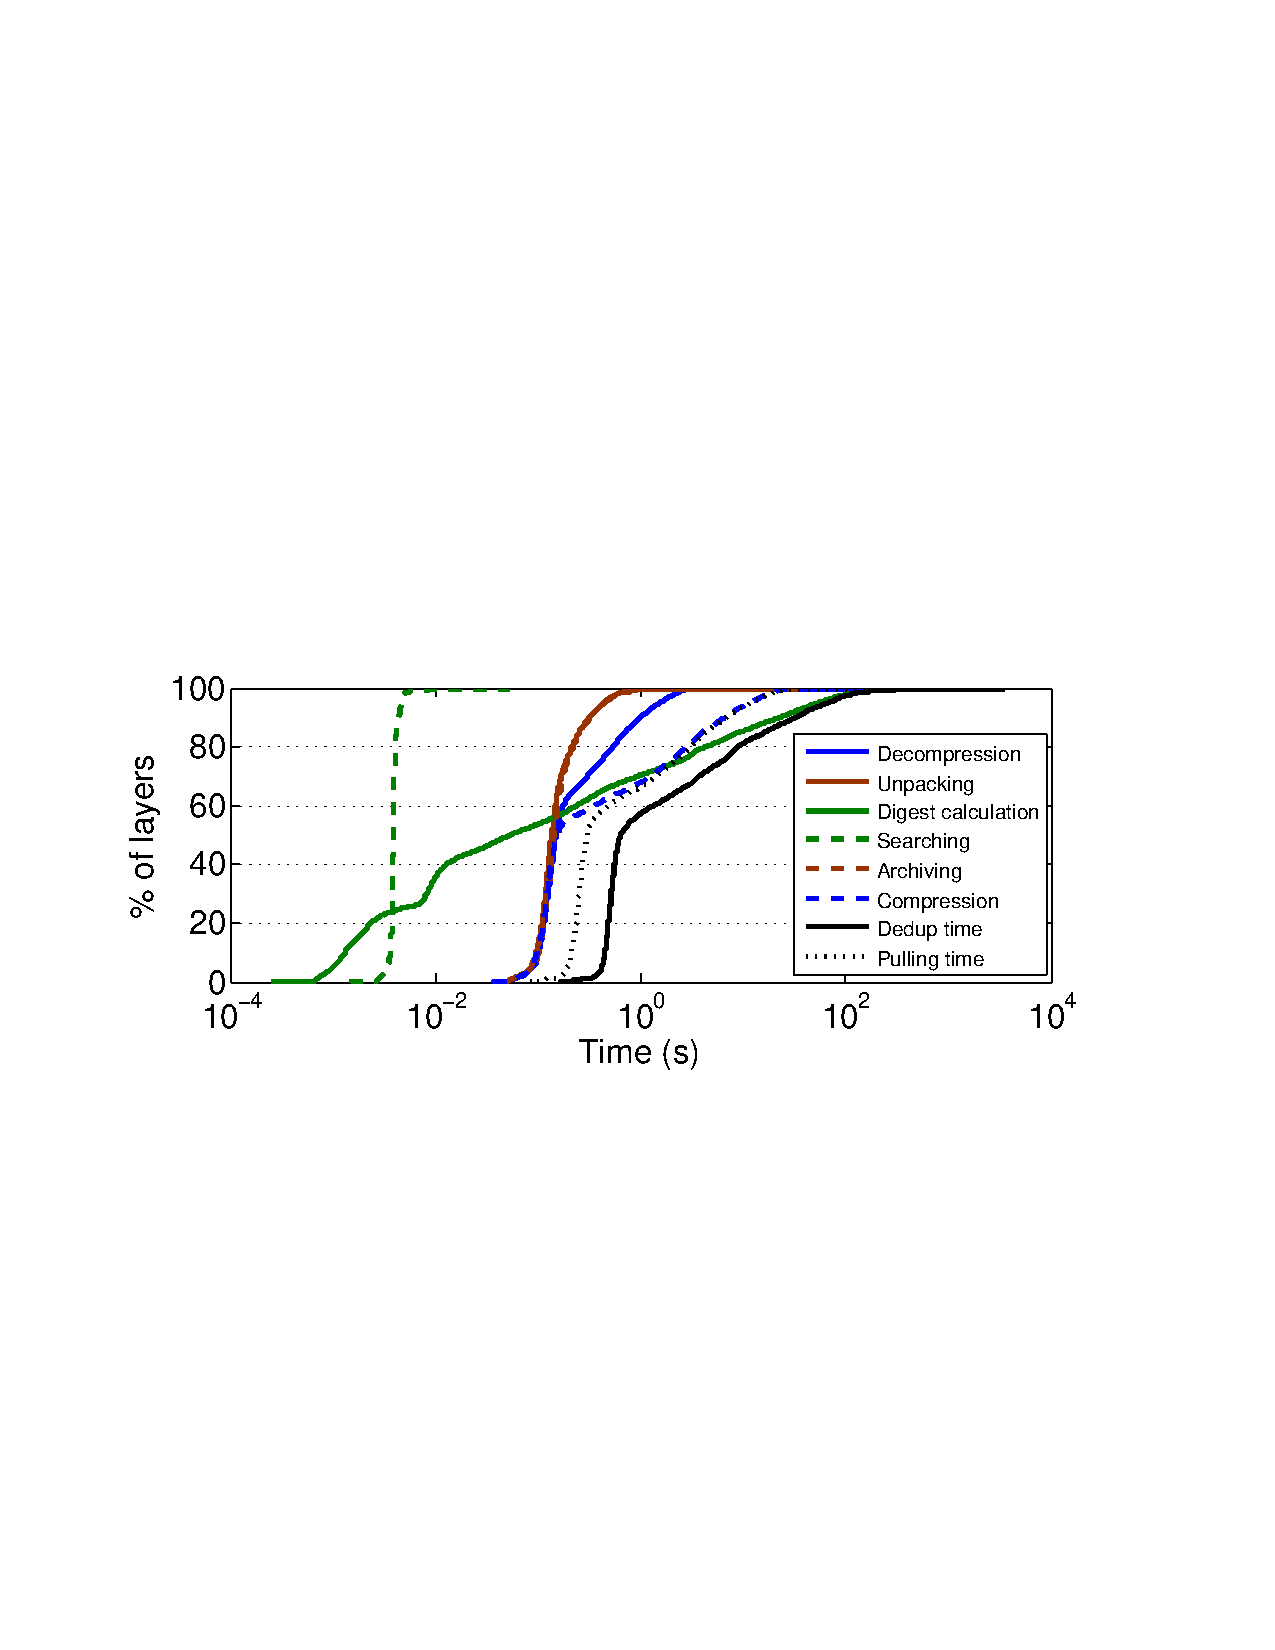
\includegraphics[width=0.5\textwidth]{graphs/res-time.pdf}
	\caption{Off-line file-level deduplication run time.}
	\label{fig:dedup-res}
\end{figure}

%
%
%%\paragraph{Hit ratios}
%%
%%\paragraph{Hit ratios with prefetching}
%%
%%%\subsection{} % what are the cost for a naive file-level deduplication
%%
%%\paragraph{Restoring performance breakdown}
%%
%%\paragraph{Simulation}
%%
%%To analyze the impact of file-level deduplication on the registry performance,
%%we conduct a preliminary simulation-based study of \sysname.
%%
%%Based on the simulation results, we estimated the overhead of \sysname\ on
%%\texttt{push} and \texttt{pull} layer request latencies.
%%
%%We then provide different suggestions on how the Docker registry can mitigate
%%the deduplication overhead.
%%
%%%%%%%%%%%%%%%%%%%%%%%%%%%%%%%%%%%%%%%%%%%%%%%%%%%%%%%%%%%%%%%%%%%%%%%%%%%%%
%%
%%
%Our simulation
%approximates several of \sysname's steps as described in Section~\ref{sec:design}.
%%
%First, a layer from our dataset is copied to a RAM disk. 
%%
%%
%%Note that there is no foreground pull or push requests since the simulation is \emph{off-line}.
%%
%The layer is then decompressed, unpacked, and the fingerprints of all files
%are computed using the MD5 hash function~\cite{MD5}.
%%
%The simulation searches the fingerprint index for duplicates,
%and, if the file has not been stored previously, it records the
%file's fingerprint in the index.
%%
%%To map a layer to its containing files, we create the layer recipe and add it
%%to a \emph{layer-to-file table}.
%%
%%The simulator then creates a file recipe.
%%
%%For each file in a layer, a layer digest
%%to its containing file content digest mapping record is also created 
%%
%%The \emph{layer-to-file table} also
%%records the file path within each layer associated with each file.
%%
%At this point our simulation does not include
%the latency of storing unique files.
%%
%To simulate the layer reconstruction during a \texttt{pull} request,
%we archive and compress the corresponding files.
%%
%%Only unique files are maintained in RAM
%%disk while the redundant copies are removed.
%%
%
%The simulator is implemented in 600 lines of Python code
%and our setup is a one-node Docker registry on a machine with 32~cores and 64\,GB of RAM.
%%
%To speed up the experiments and fit the required data in RAM
%we use 50\% of all layers and exclude the ones larger than 50\,MB.
%%
%We process 60 layers in parallel using 60 threads.
%%
%The entire simulation took 3.5 days to finish.
%%
%%The overall runtime is about 3.5 days.
%
%Figure~\ref{fig:dedup-res} shows the CDF for each sub-operation of
%\sysname.
%%
%Unpacking, Decompression, Digest Calculation, and Searching 
%are part of
%the deduplication process and together make up the Dedup time.
%%
%%\VT{@Nannan, in Figure ~\ref{fig:dedup-res} can you reorder the lines in the
%%legend so that the Searching goes after Digest calculation?}\NZ{addressed}
%%
%Searching, Archiving, and Compression
%simulate the processing for a \texttt{pull}
%request and form the Pulling time.
%%
%
%%\LR{What was the overall runtime for processing 0.9 million layers?}\NZ{addressed}
%%
%%\alicomment{How are we saving the location
%%of each file in the layer? It is not clear from the following sentences.}
%%\NZ{addressed}
%%
%%To improve searching performance, the
%%mapping table is stored in Hive database~\cite{xxx}. 
%%
%%\lrcomment{Why are we using Hive for this? It seems overkill to me, especially
%%for such small data. Even at scale, a KeyValue store would probably provide
%%better performance than clunky MapReduce-based DB.}
%%
%
%\paragraph{Push}
%
%\sysname\ does not directly impact the latency of \texttt{push} requests because
%deduplication is performed asynchronously.
%%ie the registry reliably stores a
%%copy of the layer as-is and then sends a response to the client.
%%
%The appropriate performance metric for \texttt{push} is the time it takes to deduplicate
%a single layer.
%%
%%Next, we look at the effects on \texttt{push} and \texttt{pull} latencies in
%%more detail.
%%
%%However, if there are intensive push requests while the registry is performing
%%deduplication, \sysname\ can still impact push latencies because it incurs
%%CPU, memory, and I/O overhead. %(similar to pull requests).
%%
%Looking at the breakdown of the deduplication time in
%Figure~\ref{fig:dedup-res}, we make several observations.
%
%First, the searching time is the smallest among all operations with 90\% of the
%searches completing in less than 4\,ms and a median of 3.9\,ms.
%%
%%The mapping table maintains 0.98 million layer-to-file digest mapping records. 
%%
%%\LR{Remove the following sentence? 1.7 million records is actually quite small
%%so even a single-node DB with one index is enough.}\NZ{addressed} Consider
%%that more than 1.7 million layers are stored in Docker hub and the number is
%%still increasing, it's better to choose a fast distributed database to provide
%%high searching performance and scalability.
%%
%Second, the calculation of digests spans a wide range from 5\,$\mu$s to almost
%125\,s.
%%
%%This is because the time mainly depends on the layer size, \ie the fewer and
%%smaller files a layer contains, the faster it is to compute all digests for
%%the layer.
%%
%%Typically, smaller layers contain a smaller number of smaller files, which
%%takes much less time to calculate their digests.
%%
%%While if the layer is bigger, the digest calculation overhead will be higher. 
%%
%90\% of digest calculation times are less than 27\,s while 50\% are
%less than 0.05\,s.
%%
%The diversity in the timing is caused by a high variety of layer sizes both in
%terms of storage space and file counts.
%%
%%Thus, we suggest that multiple-threading is needed to calculate the files'
%%digests simultaneously; 
%%
%%Fast CPUs as well as more powerful computing nodes are required to speed up
%%digest calculation.
%%
%Third, the run time for decompression and unpacking follows an identical
%distribution for around 60\% of the layers and is less than 150\,ms.
%%
%%Around 60\% of decompression and unpacking time are less than 0.15\,s. 
%%
%However, after that, the times diverge and decompression times increase faster
%compared to unpacking times.
%%
%%\VT{do we have some theory why?}
%%\NZ{decompressing the layers with bigger uncompressed size takes longer time.}
%%
%90\% of decompressions take less than 950\,ms while 90\% of packing time is less
%than 350ms.
%
%%Overall, we see that file digest calculation contributes a lot to the
%%overall deduplication latency especially when the layer size is big.  Moreover,
%%we see that the deduplication latency increases as the layer size grows.
%%
%Overall, we see that 90\% of file-level deduplication time is less than 35\,s
%per layer, while the average processing time for a single layer is 13.5\,s.
%%
%This means that our single-node deployment can process about 4.4\,layers/s on average
%(using 60 threads).
%%
%In the future we will work on further improving \sysname's deduplication throughput.
%%
%%In a large-scale registry deployment, this throughput can be improved
%%as more node are available to perform deduplication.
%%
%
%\paragraph{Pull} 
%
%From Figure~\ref{fig:dedup-res}
%we can see that 55\% of the layers have close compression and archiving
%times ranging from from 40\,ms to 150\,ms and both operations contribute equally
%to pulling latency.
%%
%%60\% of compression and archiving time are less than 0.15 s.
%%
%%While compression has the highest run time 80\% of compression time is less than 2.82~s. 
%%
%%\LR{Again, better to show the 90th percentile.}
%%\NZ{90\% of the compression time is less than 8\,s.}
%After that, the times diverge and compression times increase faster with an
%90\textsuperscript{th} percentile of 8\,s.
%%
%This is because compression times increase for larger layers and follow the distribution
%of layer sizes (see Figure~\ref{fig:layer-size-cdf}).
%%
%%80\textsuperscript{th} percentile of 2.82\,s.
%%
%Compression time makes up the major portion of the pull latency and is a
%bottleneck.
%%
%Overall, the average pull time is 2.3\,s.
%
%%
%%We see that archiving time and compression contributes equally to pulling
%%latency when their run time are lower than 0.15 s while compression time almost
%%equals to pulling latency when the compression time is greater than 0.15 s. 
